\section{Fremgangsmetode}

\section{Strømmåling}
For at overvåge udgangsstrømmen skal en strømmåler realiseres. Dette kan gøres ved hjælp af en shunt modstand, $R_{s}$, som yder en meget lille og veldefineret ohmsk belastning og kan holde til hele udgangsstrømmen. Når belastningen trækker en strøm, vil et lille spændingsfald forekomme over shunt modstanden, som en differensforstærker vil detektere. På figur \ref{fig:current_sense} ses schematics over strømmåleren.

\begin{figure}[h]
	\centering
	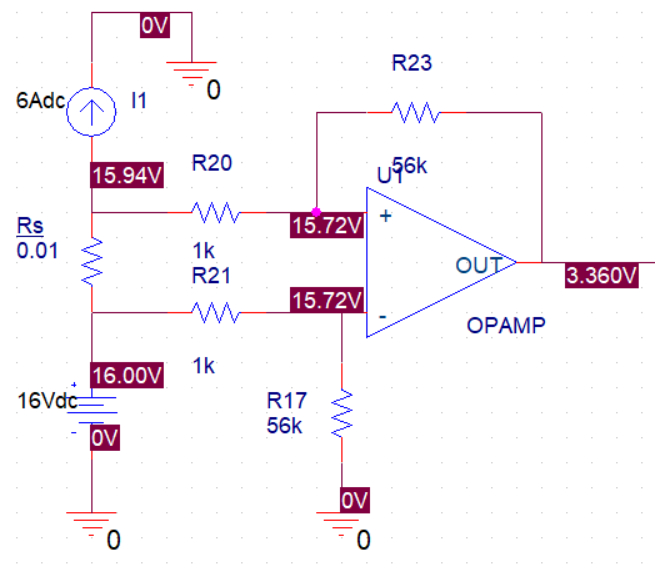
\includegraphics[width=15cm]{billeder/current_sense.png}
	\caption{Differensforstærker som strømmåler}
	\label{fig:current_sense}
\end{figure}

Med en maksimal afladestrøm $I_{out} = 6\ampere$ vælges shunt modstanden $R_{s} = 10\milli\ohm$. Det maksimale spændingsfald, $V_{s}$ over shunt modstanden bliver derfor
\begin {equation} 
V_{s} = R_{s} * I_{out} = 10\milli\ohm * 6\ampere = 60\milli\volt
\end {equation}

Afladestrømmen kan variere mellem $0\ampere$ og $6\ampere$, så spændingsfaldet vil ligge mellem $0\milli\volt$ og $60\milli\volt$. Da microcontrolleren kører på $3.3\volt$ logik med en ADC opløsning på 12 Bit, skal signalet dimensioneres til dette. Ved hjælp af en differensforstærker kan et brugbart indgangssignal til ADC'en realiseres. Forstærkeren er opbygget med en operationsforstærker koblet med positiv feedback.
\\

Den nødvendige forstærkning $A_{v}$ af signalet findes,
\begin {equation} 
A_{v} = \frac{V_{o}}{V_{s}} = \frac{3.3\volt}{60\milli\volt} = 55
\end {equation}


